\documentclass[10pt,twocolumn,letterpaper]{article}

\usepackage{cvpr}
\usepackage{times}
\usepackage{epsfig}
\usepackage{graphicx}
\usepackage{amsmath}
\usepackage{amssymb}

% Include other packages here, before hyperref.

% If you comment hyperref and then uncomment it, you should delete
% egpaper.aux before re-running latex.  (Or just hit 'q' on the first latex
% run, let it finish, and you should be clear).
\usepackage[breaklinks=true,bookmarks=false]{hyperref}

\cvprfinalcopy % *** Uncomment this line for the final submission

% Pages are numbered in submission mode, and unnumbered in camera-ready
%\ifcvprfinal\pagestyle{empty}\fi
\setcounter{page}{1}
\begin{document}

%%%%%%%%% TITLE
\title{Object Detection and Tracking Pipeline}

\author{Pranav Jain\\
Person Number: 50208349\\
UBIT: pjain4\\
%{\tt\small firstauthor@i1.org}%
% For a paper whose authors are all at the same institution,
% omit the following lines up until the closing ``}''.
% Additional authors and addresses can be added with ``\and'',
% just like the second author.
% To save space, use either the email address or home page, not both
\and
Muthuvel Palanisamy	\\
Person Number: 50246815\\
UBIT: muthuvel\\
%{\tt\small secondauthor@i2.org}%
\and
Manvijay Lather	\\
Person Number: 50200437\\
UBIT: manvijay\\
%{\tt\small secondauthor@i2.org}%
}

\maketitle
%\thispagestyle{empty}

%%%%%%%%% ABSTRACT
\begin{abstract}
   Object detection and tracking has become an integral part of Computer Vision. Efficient realization of these techniques in images and videos helped create various application in the field of automation, face detection, motion capture etc. This paper proposes an Lucas-Kanade object tracking technique initiated by Tensorflow's Object detection API and compares how this technique differs from the native tracking method employed in Tensorflow object detection.
   \end{abstract} 
%%%%%%%%% BODY TEXT
\section{Literature Review}

An optimal approach to any tracking algorithm is based on two key areas in computer vision; object detection and object tracking. While a variety of methods are available for accomplishing these techniques, not all of them prove to be effective in achieving a significant efficiency. Conventional method for accomplishing this uses techniques such as Frame Differencing, Optical flow, and Background subtraction for object detection and Point-tracking techniques, SVM and Kernel bases tracking for object tracking . A brief introduction to a some of these techniques is given below

%-------------------------------------------------------------------------
\subsection{Some Object Detection Methods}

\subsubsection{Frame Differencing}
Frame differencing suggests calculating the difference between two successive frame in an image to find the moving objects. While the idea is simple and east to implement, it is generally considered ineffective in dynamic environments where the changes in the frame of an image are not just isolated to the objects that needs to be tracked.

\subsubsection{Background Subtraction}
This techniques involves modelling the background and use that for background subtraction. We must choose a background model sensitive enough to uncover the objects in an image/frame and use that as a reference in tracking. This can be done by find the variation between frames and the reference models. Common filters like mean and median filters can be used to calculate the difference in pixel intensities. This is mainly achieved using recursive and non-recursive algorithms. A background subtraction algorithm based on frame differencing is explored in ~\cite{literaturereview}.  Similar to the previous approach, this method becomes in effective in the variation in the background becomes high. A more sophisticated method which can ignore highly changing  background will be needed for detecting objects will be required for advanced models.

\subsection{Some Object Tracking Methods}

\subsubsection{Support Vector Machine (SVM)}
SVMs apply machine learning algorithms for learning, analyzing and storing the the output as positive and negative values that represent the tracked objects in an image and objects not tracked in an image. SVMs have a wider range of application in real world, that includes but not isolated to face detection, bioinformatics, handwriting or pattern recognitions etc.

\subsubsection{Silhouette Bases Tracking approach}
This approach is helpful in tracking complex geometric shapes present in images such as hands, fingers etc. It can be done by employed by track either the boundary(Contour) of objects in an image or the shape corresponding to those objects. Contour based tracking can be achieved using gradient descent minimization technique and using state space models to trace boundaries. Shape Matching is a kind of brute force approach applied on a region of interest in a frame to identify objects that can be matched with a reference object


\subsection{Tensorflow API}

Tensorflow was originally developed by Google Brain Team to help facilitate machine learning and deep learning researches. Tensorflow's object detection model consists of a neural network trained from COCO(Common Objects in Context) dataset. It contains around 300k images of 90 commonly used objects. The library consists of 5 different models to use; classified based on their speed and accuracy of placing the bounding box (a box that encloses a detected object). We plan to use all the 5 different models and compare the results of one with the another to find the most optimal one.

\subsection{Lucas-Kanade Tracker in OpenCV}

Devoped by Bruce D. Lucas and Takeo Kanade, Lucas-Kanade Tracker uses an optical flow algorithm to track an object in subsequent frames. OpenCV incorporates a predefined function - \textit{calcOpticalFlowPyrLK()} , for implementing this algorithm, which we are planning to append to the tensorflow's object detection technique


%-------------------------------------------------------------------------
\section{Method Proposed}
Trained Neural Networks has been proven to produce better efficiency and detection models. 

Our idea is to come up with an ideal tracking method that is able to self detect object and track them. We aim to make use of tensorflow's object detection technique and the Lucas-Kanade tracker implemented using opencv library. The desire pre-trained model used to detect an object is downloaded from the Tensorflow library.

We want to experiment three different methods in achieving a tracking algorithm which are as follows

\subsection{Objection detection using Tensorflow}
In this method, we employ a detection technique using object detection function from Tensorflow. The process initiates by starting with the first frame in a video or image. The object detected is visualized using a bounding box enclosing the object. This is done by the function\textit{visualize\textunderscore boxes\textunderscore and\textunderscore labels\textunderscore on\textunderscore image\textunderscore array()}  In every successive frame, the same object detection algorithm is employed to detect the new interesting objects in the frame. In the end, detecting  objects in all the frame individually translates to an indirect object tracking method.

\subsection{Object tracking initialized by Tensorflow}

In this method, we initialize the process by starting with Tensorflow's object detection. The first part of the detects the objects of interest in the image using the pre-trained model The objects detected in the first frame is used as input for tracking in the second part.

The object detection technique employed here returns an array of bounding boxes which consists of a array of co-ordinates for boxes enclosing an object for all interesting objects and their corresponding scores. Since, all the boxes detected may not used ideal, we set a threshold to the scores to limit the number boxes.

In the next part, we use SIFT detector on the first frame of the video/ image to detect the feature points in the image. Not all points here are required for tracking. Hence, we limit them by choosing only the feature point present inside the bounding box detected from the object detection. This will give us the keypoints that can be used to track the object.

Using the feature points extracted above, we initiate the Lucas-Kanade tracking function- \textit{calcOpticalFlowPyrLK()} from openCV. The difference in the location of the object in the current frame to that in the previous frame in calculated. This is used to eliminate static objects from background by setting a threshold on the difference. 

Finally, a bounding box is drawn over the object using the \textit{visualize\textunderscore boxes\textunderscore and\textunderscore labels\textunderscore on\textunderscore image\textunderscore array()}  function from tensorflow library.

Many authors misunderstand the concept of anonymizing fosr blind
review.  Blind review does not mean that one must remove
citations to one's own work---in fact it is often impossible to
review a paper unless the previous citations are known and
available.

\subsection{Hybrid Approach}
As the name suggests, this method employs the correlation between both object detection from Tensorflow and Lucas-Kanade Tracker. The outcome visualized is to combine Tensorflow's efficiency in detection and the speed of tracking achieve by KLT algorithm. This idea is to create a fail proof technique in which the shortcomings in the KLT algorithm is balance by usage Tensorflow to detect objects periodically.

So, instead of just using the object detection technique only for initializing, we use Tensorflow to detect object for every \textbf{n} frames and pass the detected objects as input to tracker everytime. So, in short once the object detection passes the input to tracker, it waits for \textit{n} frames to detects objects again and pass the same to the tracker. This approach has a potential benefit of detecting objects that are not present in the beginning of the video. Also, it could help rectify any pitfalls in the Tracking algorithm but constantly running object detection again while maintaining speed.

%------------------------------------------------------------------------
\section{Experimental Analysis and Result}

We have tested all the three approaches discusses earlier with a few hand-picked videos and image sets. A link to the the original output files are in ~\cite{Videolink}. Also, we have compared the time taken to track an object in a video using three different approaches discussed in the previous sections of this report. Please find below the detailed analysis

\subsection{Object detection using tensorflow}  

When we implemented the first algorithm (Object Detection using Tensorflow) on the videos, we found out that it misses on detecting objects later in the video which were detected in the initial frames of the video. We tried it on a set of test images taken by a CCTV camera and it gave us the same result. As far as the running time is concerned this approach almost took twice as long as the other two algorithms. \textit{See Figure 1}.

    %% Inluding the images
\begin{figure}
\includegraphics[width=\linewidth]{Detection.jpg}
\caption{Detection using Tensorflow for a video }
\end{figure}

This algorithm was run on a series of test images as well, screenshots of which are shown in \textit{Figure 2}

\begin{figure}
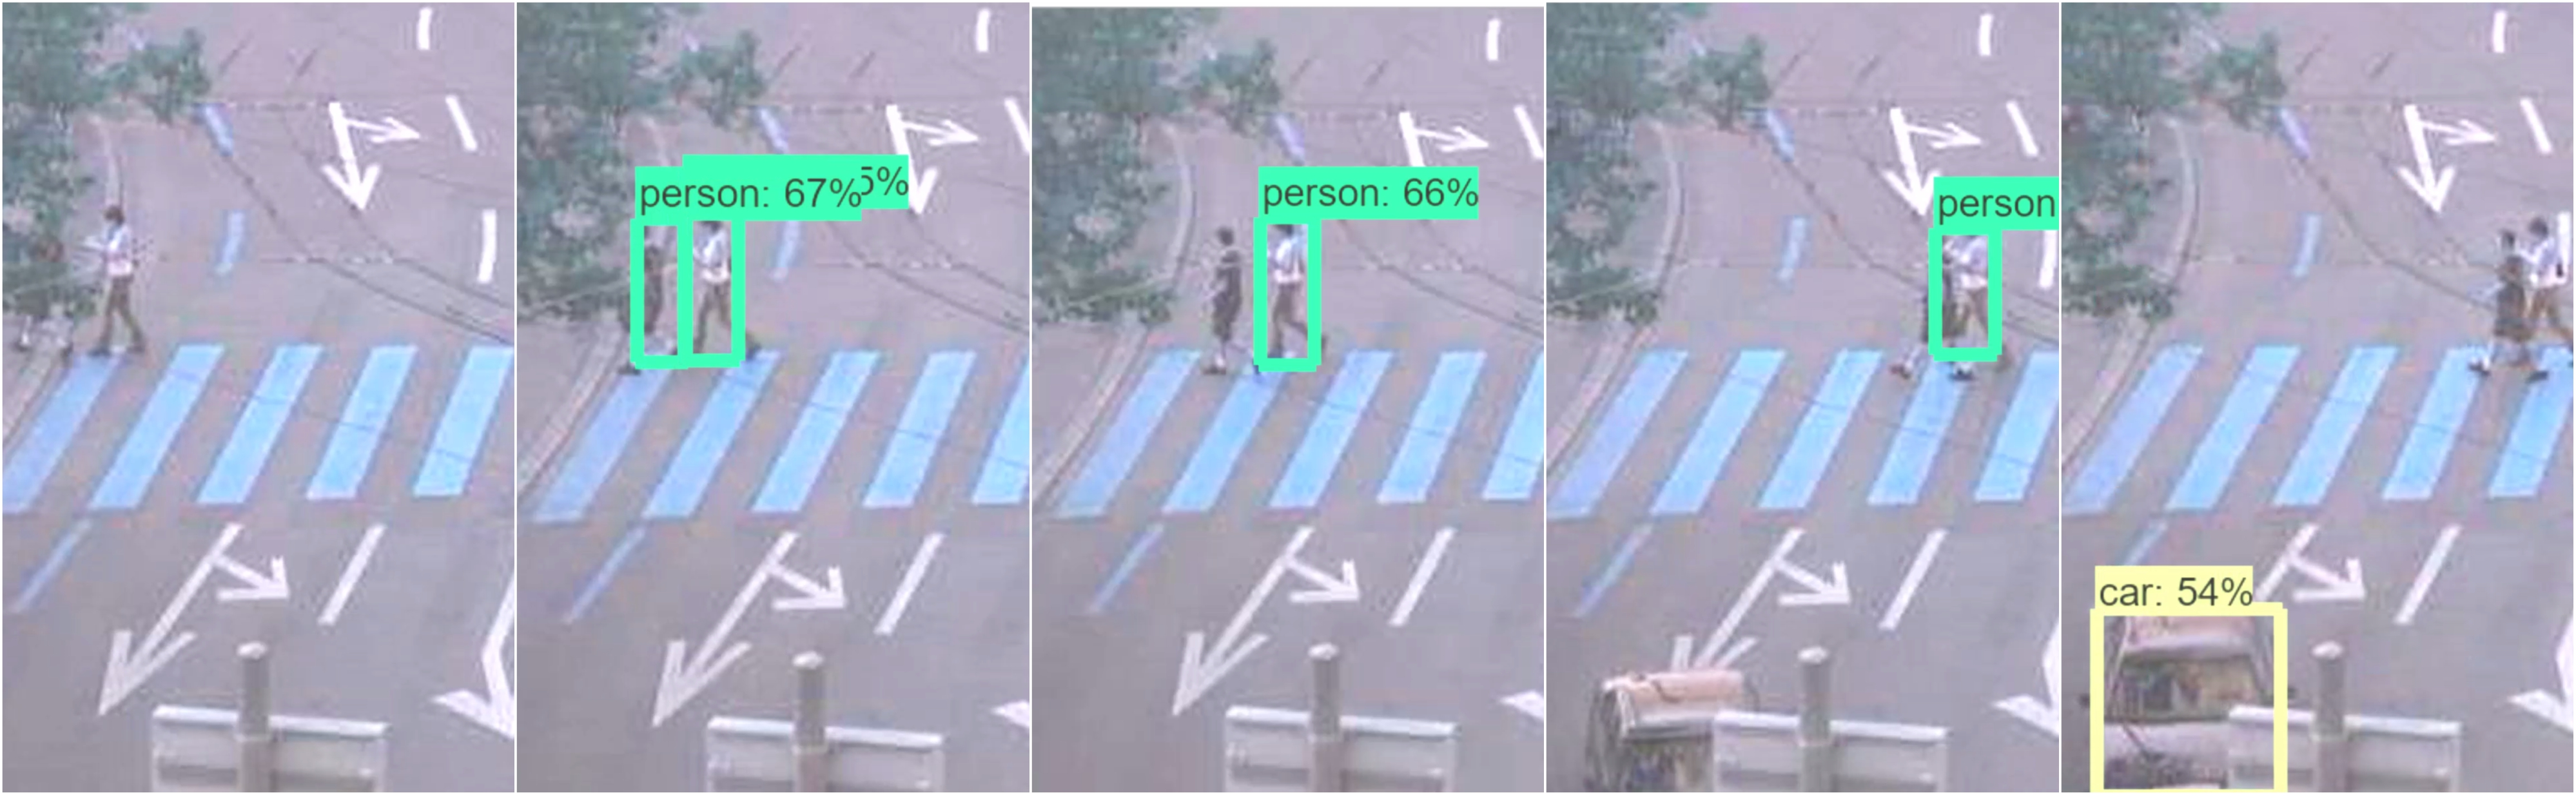
\includegraphics[width=\linewidth]{Detection_images.jpg}
\caption{Detection using Tensorflow for a sequence of images}
\end{figure}

\textbf{Advantages:}

•	This is the backbone of the other two approaches.
•	People in the machine learning community is aware of Tensorflow which means More minds solving problems hence more shoulders to stand upon!

\textbf{Disadvantages:}

•	When implemented on videos, doesn’t always detect the object which was detected in one of the previous frames of the same video. 
•	Takes more time.

\subsection{Object tracking initiated by Tensorflow}  

On implementing this algorithm, we got quicker results than the first approach, almost half the time. The other positive point of this algorithm we observed was that it never lost track of the object which was tracked in the initial frames of the video. However, there is a limitation in this algorithm. The box enclosing the feature points of the detected objects keep reducing in the size as the video progresses. The reason for that diminishing box is the lesser number of feature points left inside the box after comparing two consecutive frames.\textit{ See Figure 3}.

\begin{figure}
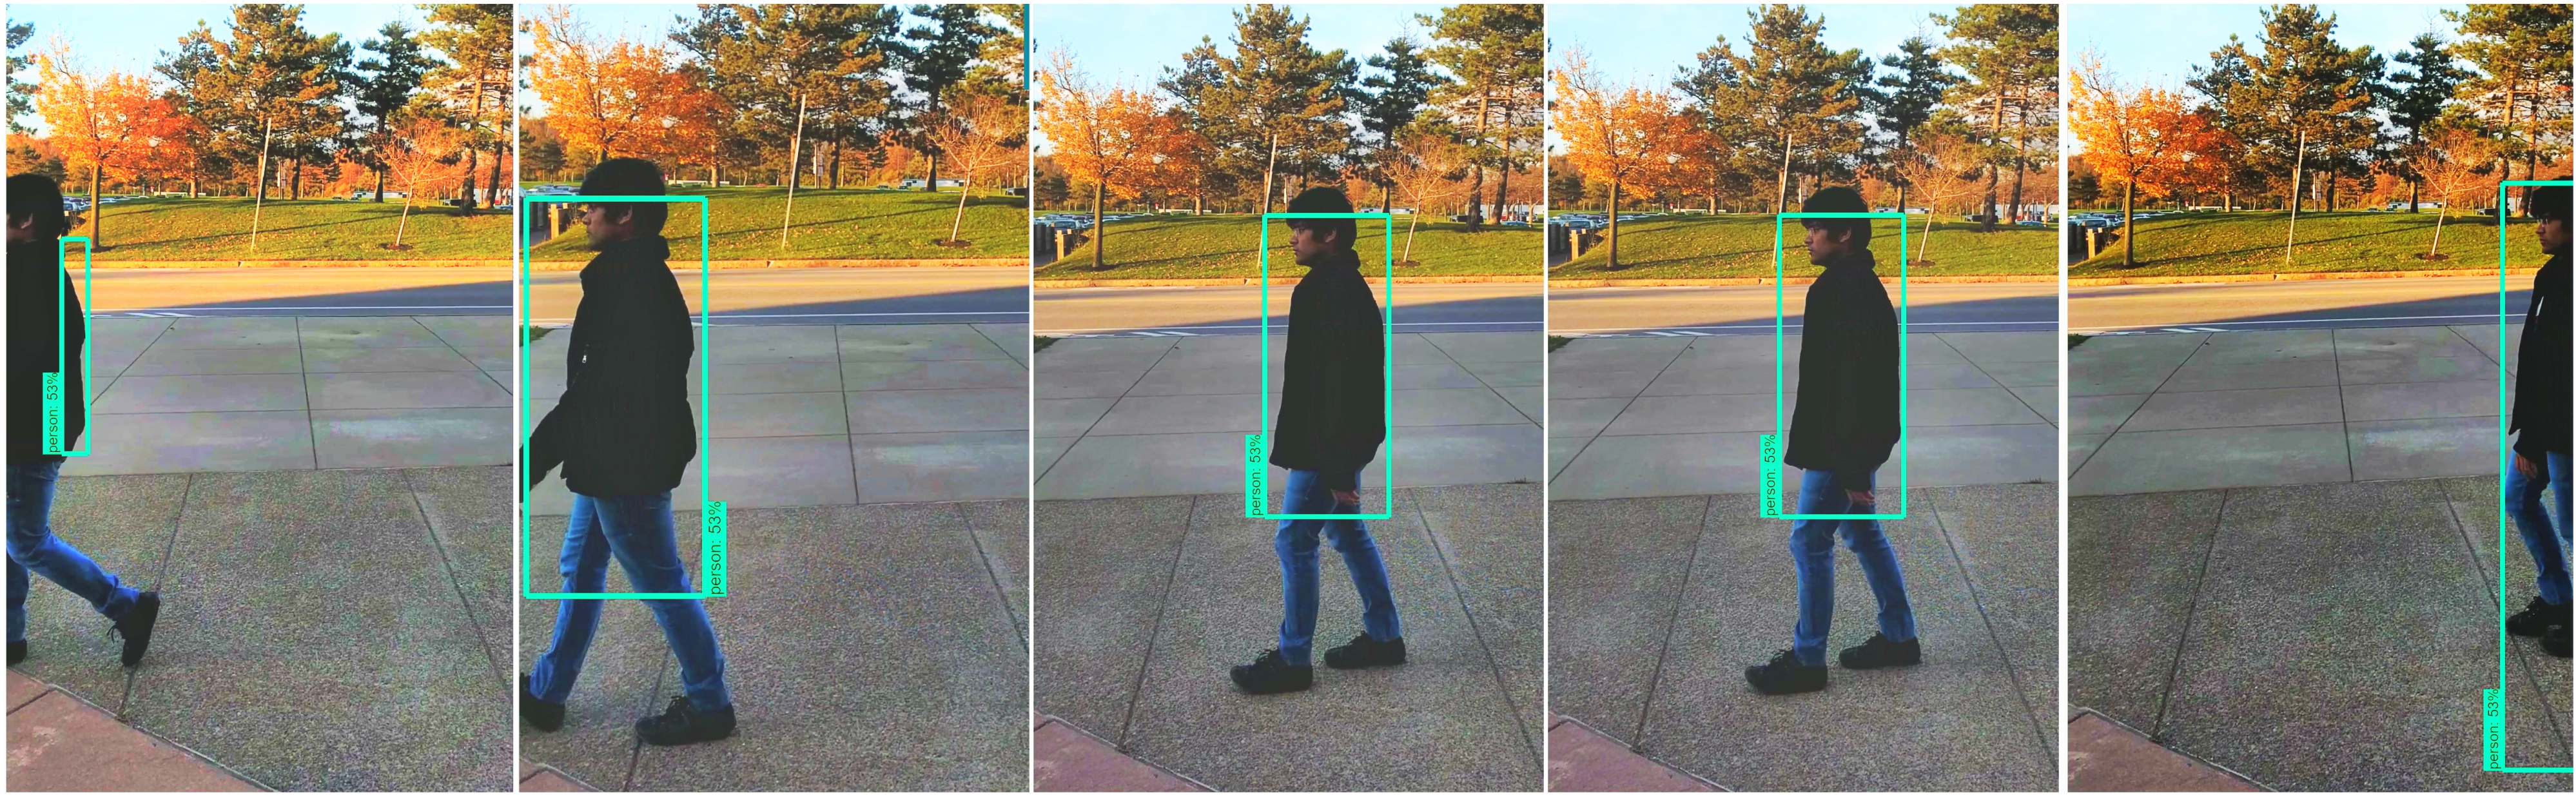
\includegraphics[width=\linewidth]{Tracking.jpg}
\caption{Object Tracking in a video initiated by Tensorflow}
\end{figure}

This algorithm was run on a series of test images as well, screenshots of which are shown in \textit{Figure 4}.

\begin{figure}
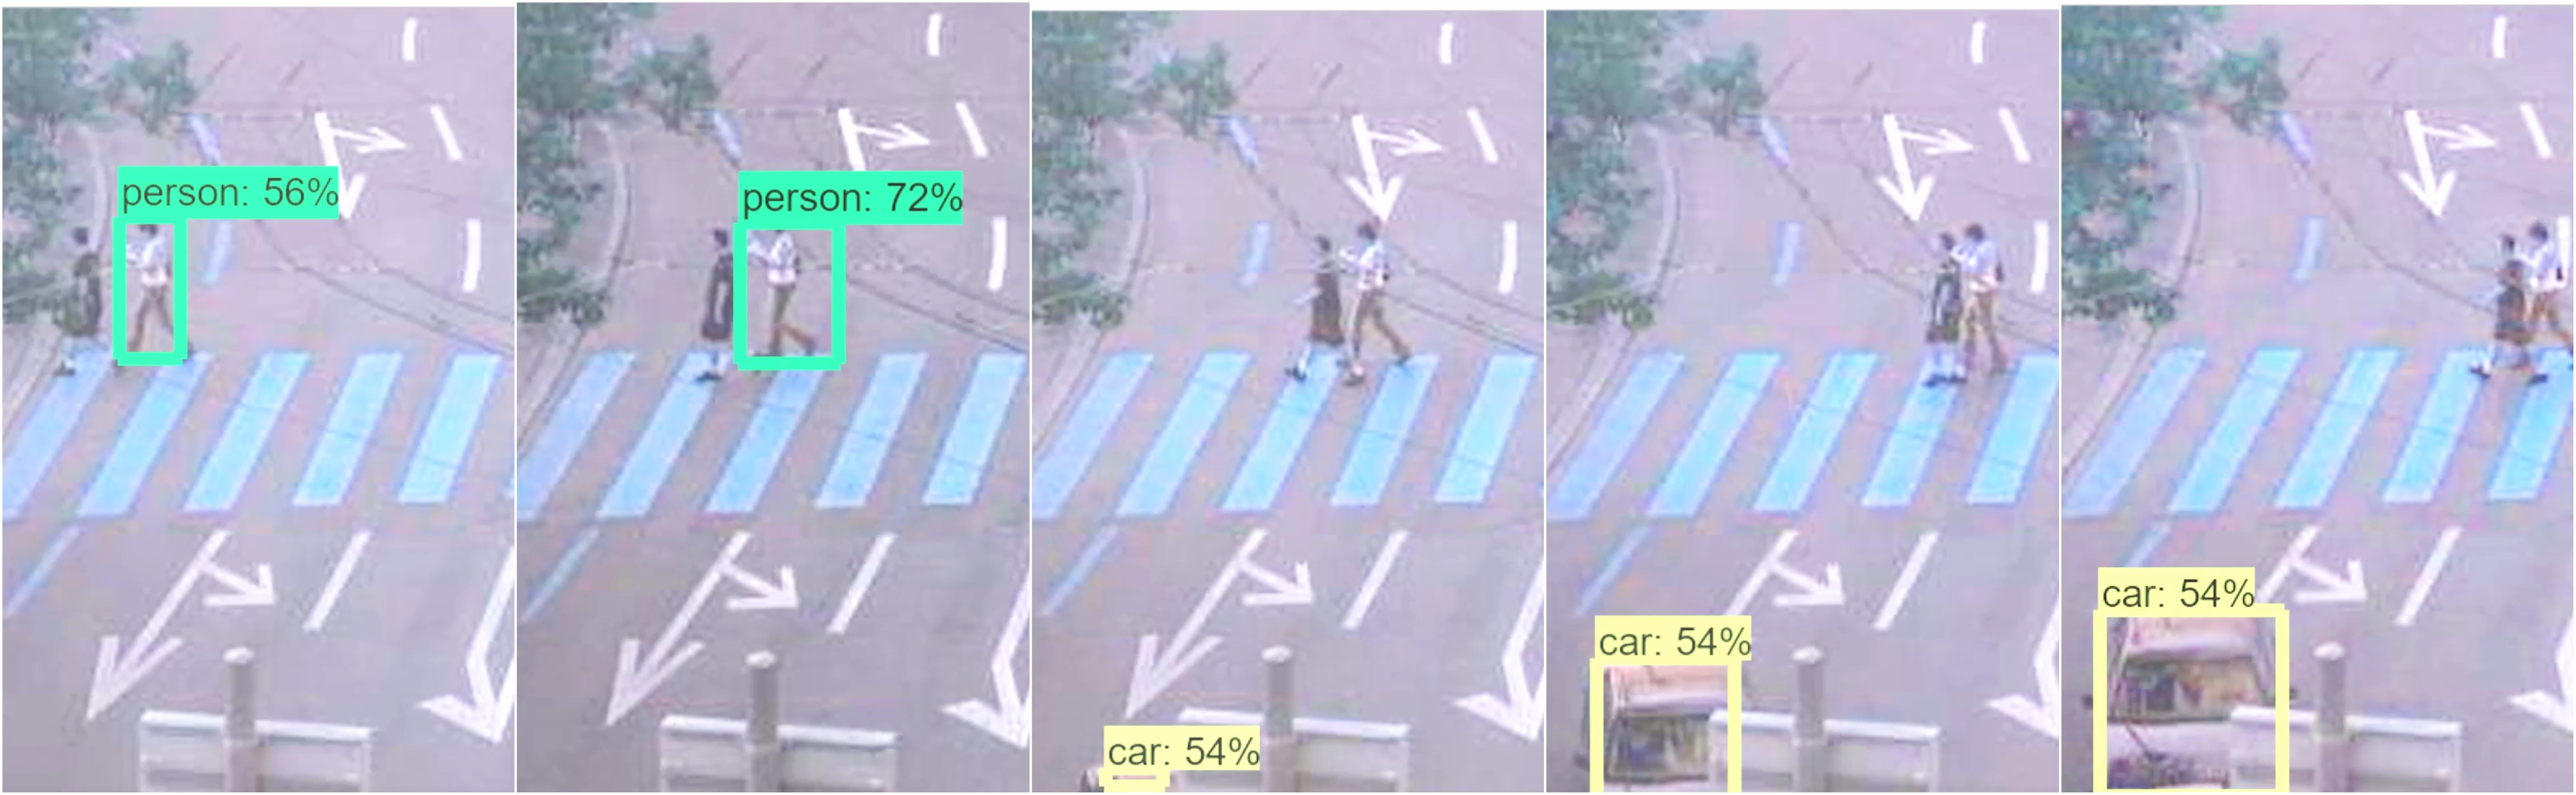
\includegraphics[width=\linewidth]{Tracking_images.jpg}
\caption{Object Tracking in a sequence of images initiated by Tensorflow}
\end{figure}

\textbf{Advantages:}

•	It’s substantially faster than TensorFlow approach and marginally faster than Hybrid approach.
•	It keeps track of the object detected in one frame till the end of the video.

\textbf{Disadvantages}

•	Rely on TensorFlow to detect an object before it can track that object throughout the video.
•	Decrease in size of the box enclosing the feature points of the detected object as the time passes or in other not enclosing all the feature points of the detected object after a few frames.
 
\subsection{Hybrid Approach}  

This approach keeps the best elements from the previous algorithms. It’s almost as fast as second approach and can be trusted with detecting new objects in the middle of the video (a trait shown by first algorithm). However, the only limitation it has is its over reliance on Tensorflow which leads to not detecting objects once Tensorflow is unable to detect the object. It’s an upgrade on tracking algorithm as it detects algorithm even in the intermediate frames of the video but loses its edge if TensorFlow fails to detect it in the frame where this algorithm uses TensorFlow for detection. \textit{See Figure 5}.

    %% Inluding the images
\begin{figure}
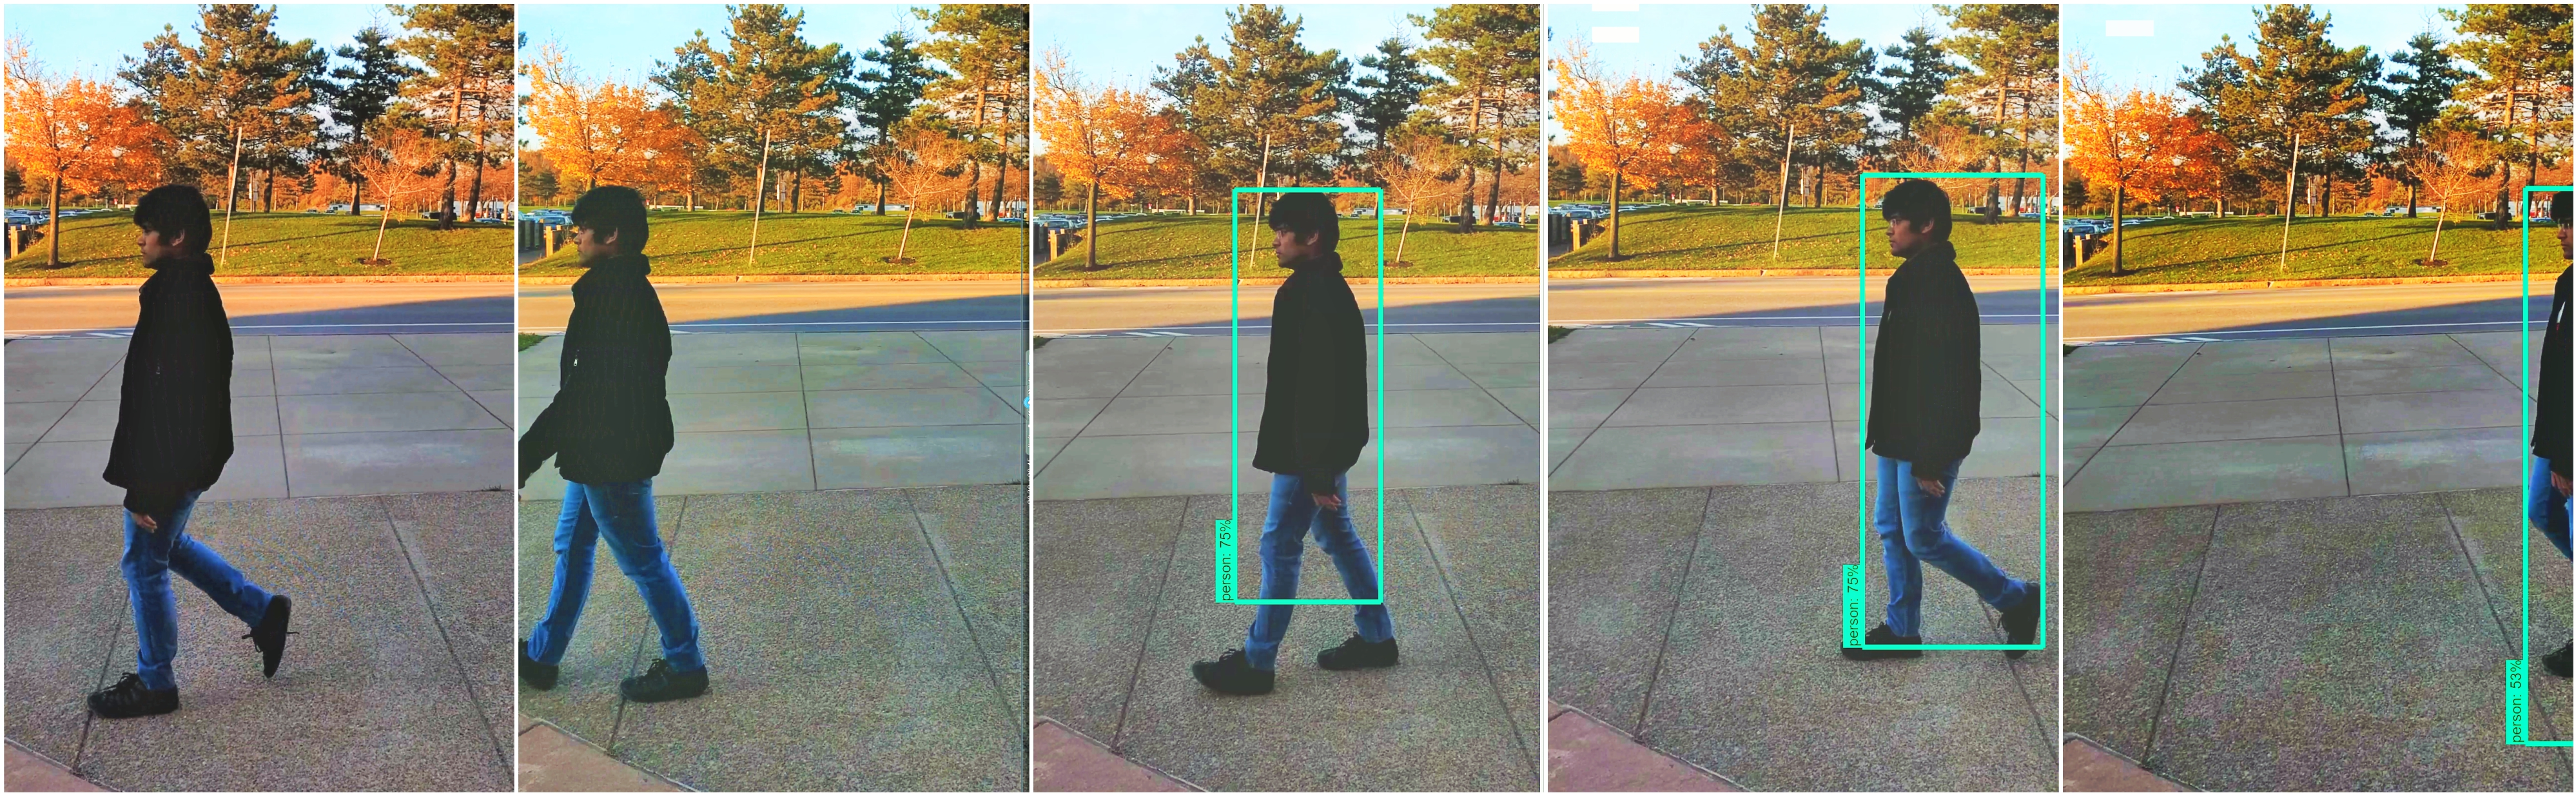
\includegraphics[width=\linewidth]{Hybrid.jpg}
\caption{Hybrid approach on a video}
\end{figure}

This algorithm was run on a series of test images as well, screenshots of which are shown in \textit{Figure 6}.

    %% Inluding the images
\begin{figure}
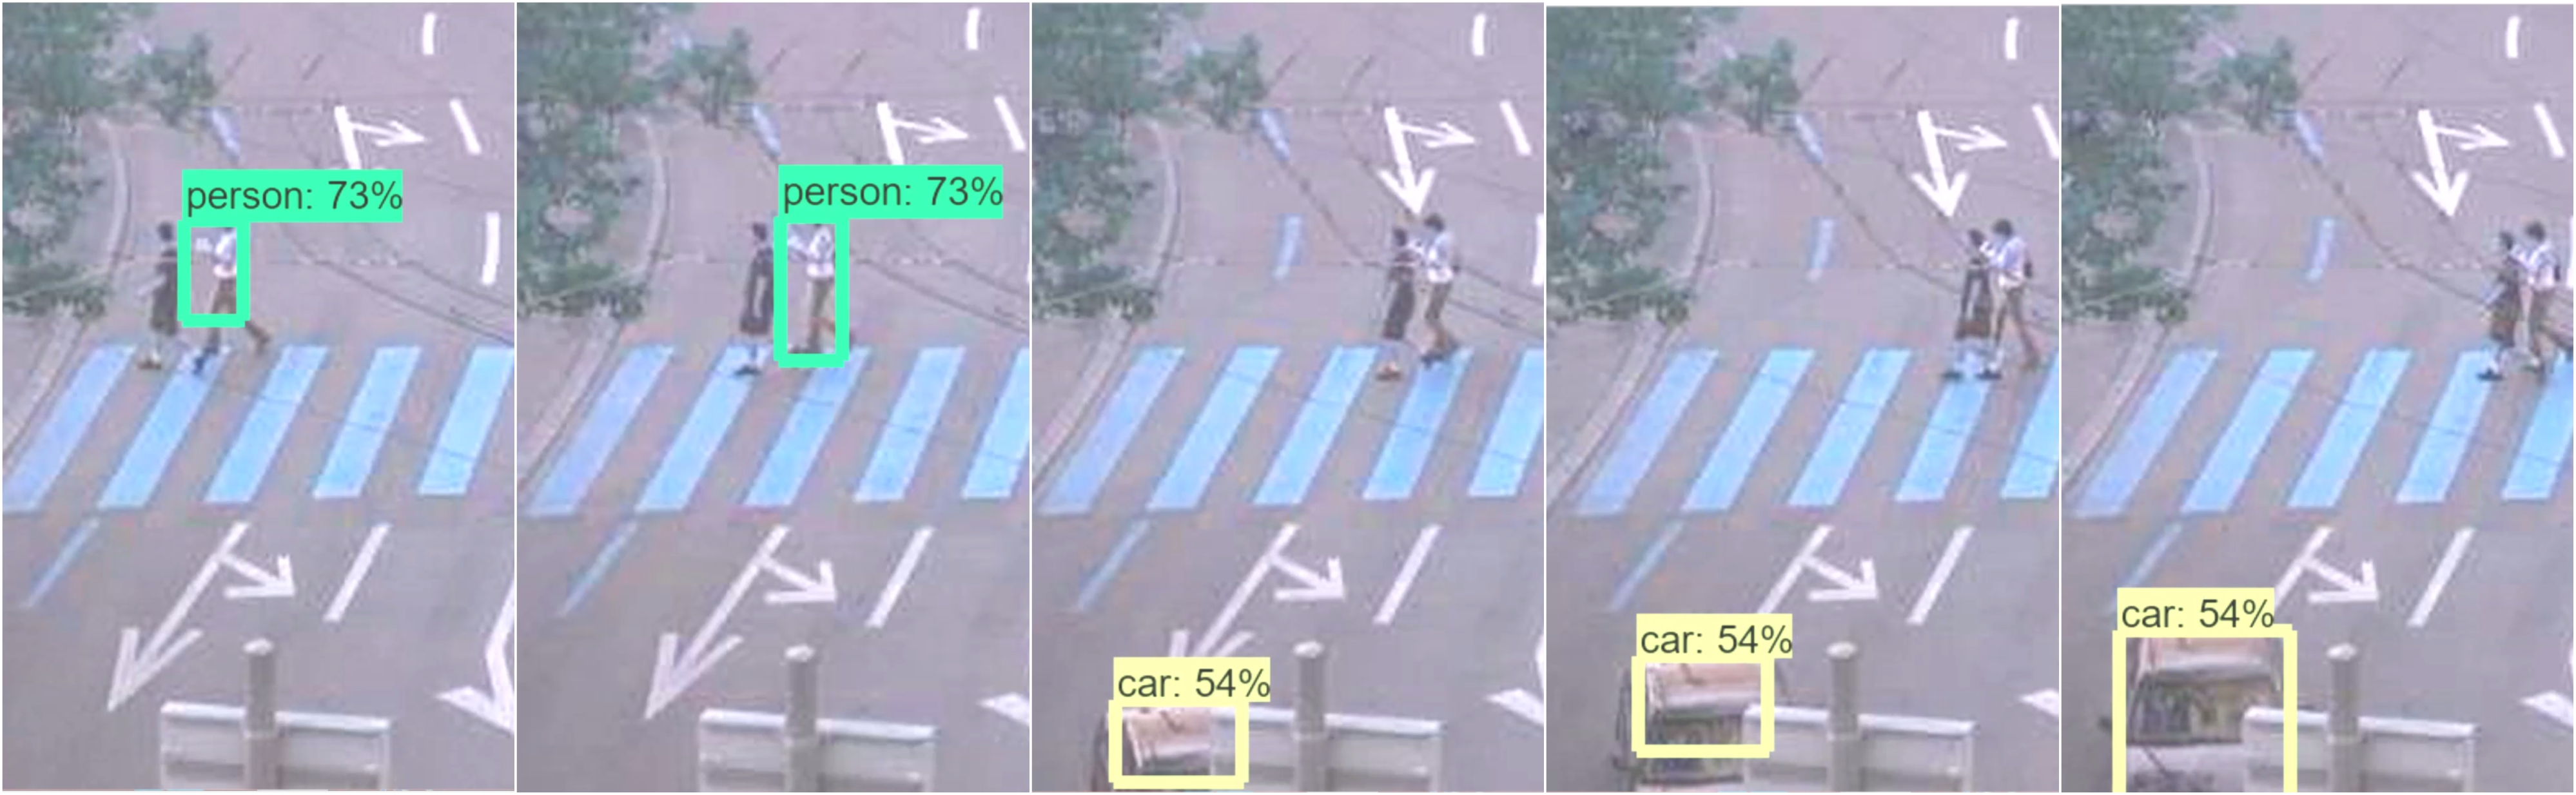
\includegraphics[width=\linewidth]{Hybrid_images.jpg}
\caption{Hybrid approach on a sequence of images}
\end{figure}

\textbf{Advantages:}

•	Faster than TensorFlow/Object Detection approach.
•	More efficient than Tracking and Detection approach.

\textbf{Disadvantages:}

•	Rely on TensorFlow to detect an object before it can track that object for next n frames.

\subsection{Comparison of different methods}

\textbf{What does this Graph in Figure 7 represent?}

The graph shown in \textit{Figure 7} represents the data we gathered after implementing these three algorithms on 3 different videos of same length, i.e. 3 seconds each.  
X-axis: Name of the video.
Y- axis: Time in seconds.


    %% Inluding the images
\begin{figure}
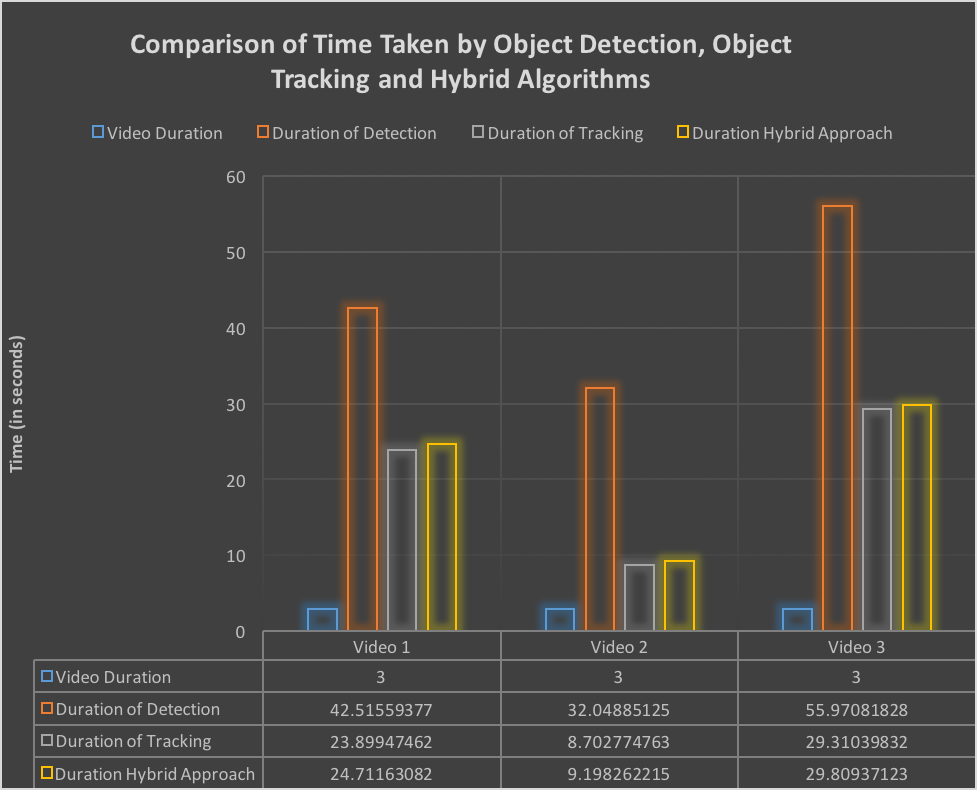
\includegraphics[width=\linewidth]{Graph.png}
\caption{Graph of Time Vs Technique}
\end{figure}
  
 
%-------------------------------------------------------------------------

\section{Conclusion and Future Work}
We will be resolving the shortcomings of our work in the future. To begin with, we will be reducing the dependency on Tensorflow for object detection by look at other alternatives. The primary reason for this is to have zero chance of error while detecting objects. Tensorflow though faster and effective most of the time, it fails to detect objects at certain frame which when coinciding with the object detection frame, can prove to be a failure in the tracking process.

As mentioned earlier, hybrid approach, though proving to be better comparitvely, it does not meet the excpectation that we expected. This is because the sweet spot for reinitializing object detection varies for different videos. Thus, this approach has too much dependency on Tensorflow. We will work on designing an algorithm to detected the ideal frame to initiate object detection in the hybrid approach. Also, a different objection detection technique as suggested above might make the hybrid approach robust.

Also, we would like to explore the possibility of running SIFT detector only inside the bounding box of the detected region of the object and see if it produces a postive impact on the speed on our model.



%-------------------------------------------------------------------------
\begin{thebibliography}{9}
\bibitem{research1} 
https://research.googleblog.com/2017/06/
supercharge-your-computer-vision-models.html
 
\bibitem{HW} 
http://16720.courses.cs.cmu.edu/hw/hw3.pdf
 
\bibitem{research} 
https://towardsdatascience.com/building-a-real-time-object
-recognition-app-with-tensorflow-and-opencv-b7a2b4ebdc32

\bibitem{literaturereview}
Rupali S.Rakibe, Bharati D.Patil.
\textit{Background Subtraction Algorithm Based Human Motion Detection}. 
International Journal of Scientific and Research Publications, May 2013

\bibitem{Videolink} 
https://drive.google.com/drive/folders/1DNHOEnZ2hg9FvYhQ7i9tk-PC6b3fAjAF

\end{thebibliography}


%-------------------------------------------------------------------------



%-------------------------------------------------------------------------
\


{\small
\bibliographystyle{ieee}
\bibliography{egbib}
}

\end{document}
